\begin{figure}[ht] 
 	\centering 
 	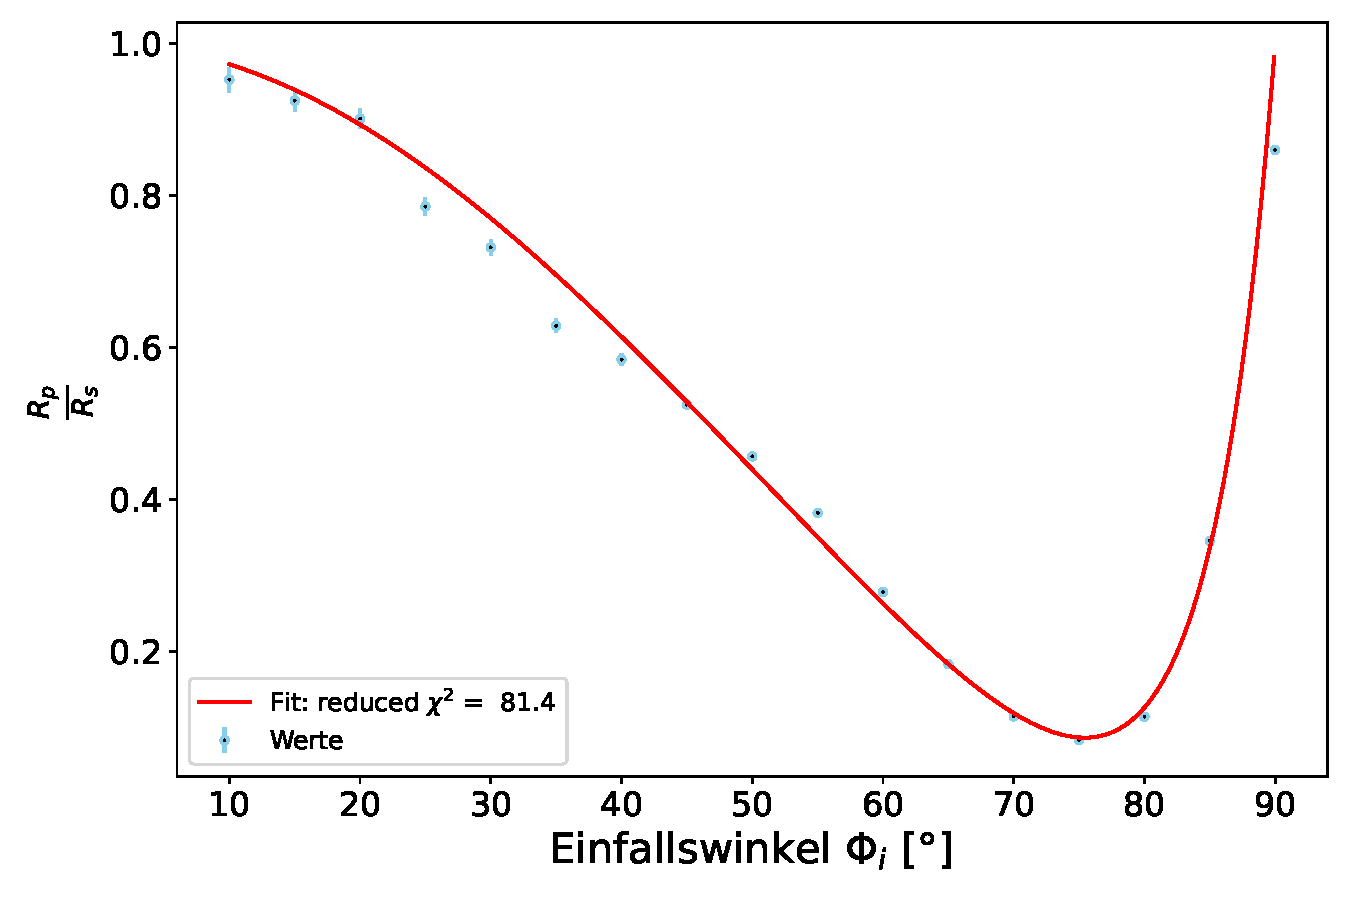
\includegraphics[width= 0.65 \textwidth]{Fits/Rp_Rs_Cu_Fit.pdf} 
	\caption{Rp Rs Cu, Fit} 
 	\label{fig:Rp Rs Cu, Fit} 
\end{figure}
 
\begin{table}[ht] 
	\centering 
	\caption{Rp Rs Cu, Fit Parameter Tabelle} 
	\label{tab: Rp Rs Cu, Fit Parameter Tabelle}
	\begin{tabular}{|l|c|}
		\hline
		Parameter Name	&	Wert \\ \hline
		n	&	 3.222 $\pm$  0.077\\ \hline
		kappa	&	-1.9785 $\pm$  0.0139\\ \hline
	\end{tabular} 
\end{table}
 
\begin{table}[ht] 
	\centering 
	\caption{Rp Rs Cu, Messwerte Tabelle} 
	\label{tab: Rp Rs Cu, Messwerte Tabelle}
	\begin{tabular}{|c|c|}
		\hline
		Einfallswinkel $\Phi_i$ [°] 	&	 $\frac{R_p}{R_s}$\\ \hline
		90.0 $\pm$ 0.2 	&	 0.860 $\pm$ 0.004 \\ \hline
		85.0 $\pm$ 0.2 	&	 0.347 $\pm$ 0.002 \\ \hline
		80.0 $\pm$ 0.2 	&	 0.116 $\pm$ 0.003 \\ \hline
		75.0 $\pm$ 0.2 	&	 0.086 $\pm$ 0.003 \\ \hline
		70.0 $\pm$ 0.2 	&	 0.117 $\pm$ 0.003 \\ \hline
		65.0 $\pm$ 0.2 	&	 0.186 $\pm$ 0.001 \\ \hline
		60.0 $\pm$ 0.2 	&	 0.281 $\pm$ 0.004 \\ \hline
		55.0 $\pm$ 0.2 	&	 0.385 $\pm$ 0.005 \\ \hline
		50.0 $\pm$ 0.2 	&	 0.459 $\pm$ 0.006 \\ \hline
		45.0 $\pm$ 0.2 	&	 0.527 $\pm$ 0.006 \\ \hline
		40.0 $\pm$ 0.2 	&	 0.587 $\pm$ 0.007 \\ \hline
		35.0 $\pm$ 0.2 	&	 0.631 $\pm$ 0.009 \\ \hline
		30.0 $\pm$ 0.2 	&	 0.734 $\pm$ 0.011 \\ \hline
		25.0 $\pm$ 0.2 	&	 0.787 $\pm$ 0.011 \\ \hline
		20.0 $\pm$ 0.2 	&	 0.902 $\pm$ 0.013 \\ \hline
		15.0 $\pm$ 0.2 	&	 0.926 $\pm$ 0.014 \\ \hline
		10.0 $\pm$ 0.2 	&	 0.953 $\pm$ 0.016 \\ \hline
	\end{tabular} 
\end{table}
 
